\chapter{Solution}

Based on the decisions described in the design chapter, regarding both the architecture and technological choices, development on the system envisioned in the previous chapter, can now begin.
This solution should help with reaching a conclusion to the problem statement, and whether the system actually does this, will be explored in \autoref{sec:conclusion}, Conclusion.

The solution chapter will elaborate on the specifics of the implementation of the solution.
The following does not describe the full implementation, but rather a selection of the most interesting aspects of the implementation.

The complete source code for the project can be found on the associated GitHub Repository: \url{https://github.com/aau-hcl-p5/main}

\section{Structure of Codebase}
The codebase is twofold, where one part is for object detection and the other part is for movement and interaction with the motors.
\todo{figure out whether the python part also does the calibration or not}
The object detection part, which is run on a Raspberry Pi, is written in Python 3{.}7, and the movement processing is handled by the NXT and is written i C, version C90 with GNU-extensions.


\subsection{Object Detection}
The codebase is seperated into modules with the intent of creating a system where each module can be exchanged based on different contexts and further development.
For the project, the following modules are used:
\begin{itemize}
	\item Object Localization Algorithm
	\item Output / Communication
	\item Input / Webcam
\end{itemize}

These are all utilized by a controller class, called \texttt{FlatController}, that ties the solution together, which has the signature shown in snippet~\ref{lst:FlatControllerInit}.
\begin{lstlisting}[language=Python,label={lst:FlatControllerInit},caption={Initialization method of the \texttt{FlatController} class}]
def __init__(self,
	algorithm: Callable[[np.ndarray], Vector],
	video_controller: webcam.VideoController,
	output_devices: Union[OutputDevice, List[OutputDevice], None] = None,
	) -> None:
	"""
	Initializes the controller
	:param output_devices: The device to send data to
	:param algorithm: The algorithm to use for image processing
	:param video_controller: The controller handling the input video
	"""
\end{lstlisting}

The order of the parameters doesn't correspond to the order of relevance, but rather is a requirement as two of the parameters have default arguments.
This method takes, as the signature shows, a function, \texttt{algorithm} with an array as input and a vector as output.
This array is the array of pixels in a given frame.
The intent of this algorithm is to take a given frame, and localize the target within the frame.


\todo{implement the video output debug to actually be what i've written below}
The \texttt{output\_devices} parameter is a class that handles transmitting the location data to the NXT, but this can be overwritten to use a video feed as output as well, with the intent of debugging. 
This argument can either be a singular \texttt{OutputDevice} or multiple, which is relevant when the user both wants to debug but also transmit the information to the NXT device.


\todo{maybe change the capture\_type to also be either a class or a function, so we follow the same paradigm of coding all the way through}
Finally, the \texttt{capture\_type} parameter specifies which device the video feed should be received from.
By default this should be a camera feed, but it might be relevant to use a specific video file in some contexts, for instance when doing tests.


The controller is initialized in the \texttt{main.py} file, which is the entry point when running the program, often from the commandline. The relevant arguments are shown in snippet~\ref{lst:MainHelp}.
\begin{lstlisting}[label={lst:MainHelp},caption={The help message of the commandline interface}]
$ python3 main.py --help
usage: main.py [-h] [-a [name]] [-d]

Run the object detection part of the F.L.A.T system

optional arguments:
-h, --help            show this help message and exit
-a [name], --algorithm [name]
Choose which algorithm to run [GOTURN, YOLO, ZONE_AVG, OBJ_FILL]. default='obj_fill'
-d, --debug           Whether to run in debug mode. whether to show video feed
\end{lstlisting}
\todo{make sure these are still up to date when finishing the project, also image, bellow it isn't as Teknight created a new algorithm- but yeah}
Figure~\ref{fig:pythonClasses} shows the dependencies of each of the actual packages, and how each module is split up, into multiple packages or files.

\begin{figure}[H]
	\centering
	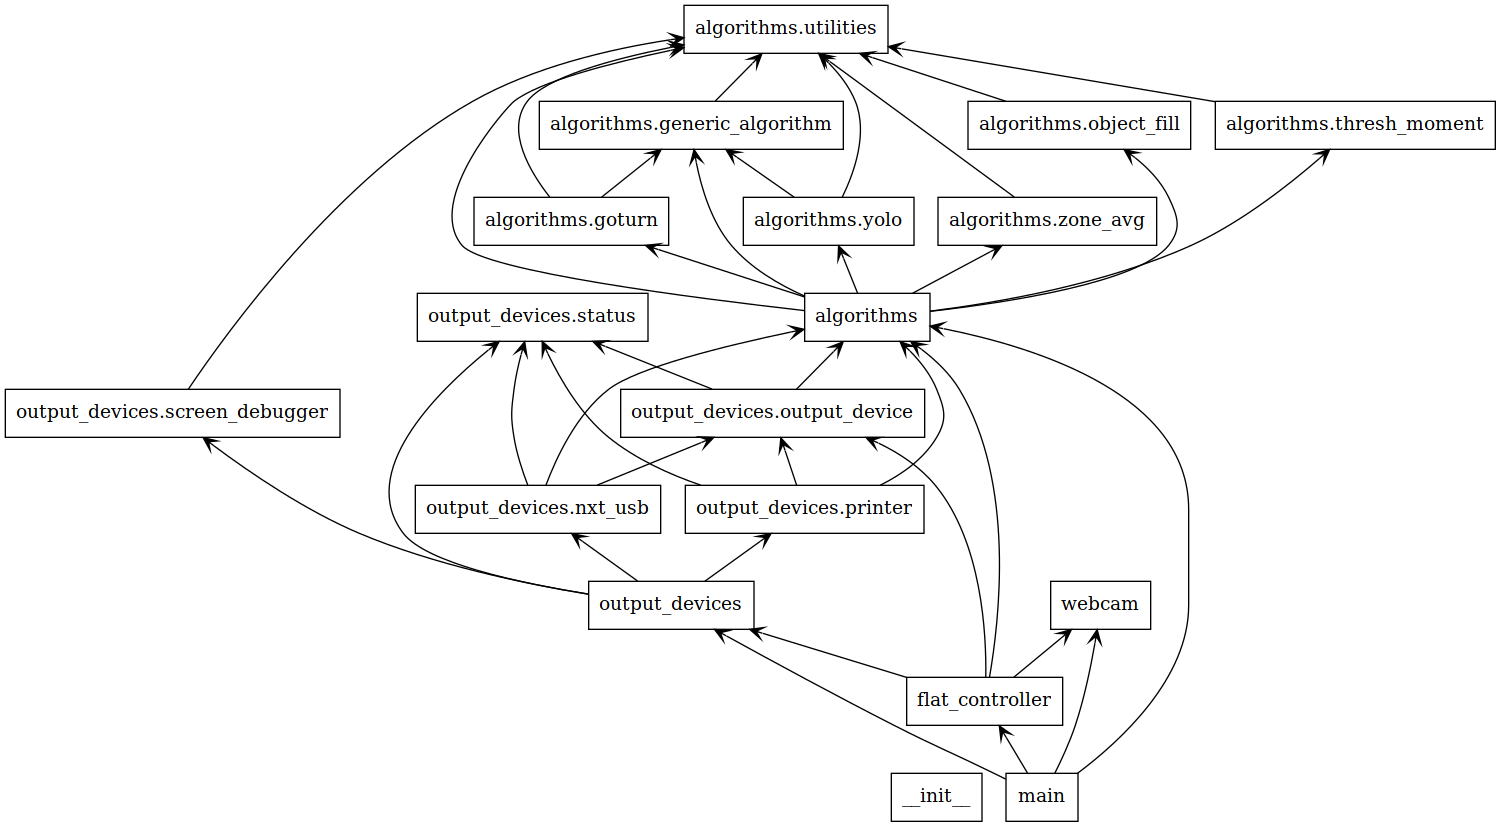
\includegraphics[width=\textwidth]{5.Solution/images/python_packages.png}
	\caption{The dependencies of the packages of the project{.} Image generated with pyreverse\cite{pyreverse}}
	\label{fig:pythonClasses}
\end{figure}


The project also contains functions for calibration, as seen on figure~\ref{fig:pythonClasses}, which will be covered in section~\ref{sec:calibration}.


\subsection{Movement}
The codebase is not in the same way seperated into modules, in a direct way, due to the design of the language. However the solution is divided into multiple file with distinct responsibilities.

\begin{itemize}
	\item \texttt{tasks}
	\item \texttt{usb}
	\item \texttt{display}
	\item \texttt{movement}
	\item \texttt{calibration}
\end{itemize}

the \texttt{tasks.c} can be seen as the primary file of the project, which creates all the tasks that the scheduling system enforces.
The code in snippet~\ref{lst:taskDecl} piece of code declares the tasks, but the specific aspects of each tasks, will be covered more indepth in section~\ref{sec:scheduling}
\begin{lstlisting}[language={c},label={lst:taskDecl},caption={Declaration of tasks, counters and events}]
/* OSEK declarations */
DeclareTask(ReceiveData);
DeclareTask(UpdateDisplay);
DeclareTask(ToggleLaser);
DeclareTask(MoveMotors);

DeclareCounter(SysTimerCnt);

DeclareEvent(MoveMotorsOnEvent);
DeclareEvent(MoveMotorsOffEvent);
DeclareEvent(LaserOnEvent);
DeclareEvent(LaserOffEvent);

DeclareResource(USB_Rx);
\end{lstlisting}
\todo{update above}
Rec


This file is not manually run, so less can be set about the overall principles of how it is run, as this is handled by the NXT-OSEK operating system, however the dependencies still seem relevant, which are detailed in figure~\ref{fig:CClasses}
\todo{insert picture here when we are done - i don't want to spend time creating one}


Each of these files and modules will be explained in-depth throughout this chapter, and explain value of each.

\

\section{Python} \label{pythonstructure}
The Python part of the project is separated into multiple modules.
The intention of a modular structure is to allow for a system that can be easily modified, based on the specific context.

For the project, the following modules are used:
\begin{itemize}
	\item Object Localization Algorithm
	\item Output / Communication
	\item Input / Webcam
	\item Calibration
\end{itemize}

\autoref{fig:pythonClasses} shows the dependencies of each of the actual packages, and how each module is split up, into multiple packages or files.

\todo{Update this}
\begin{figure}[H]
	\centering
	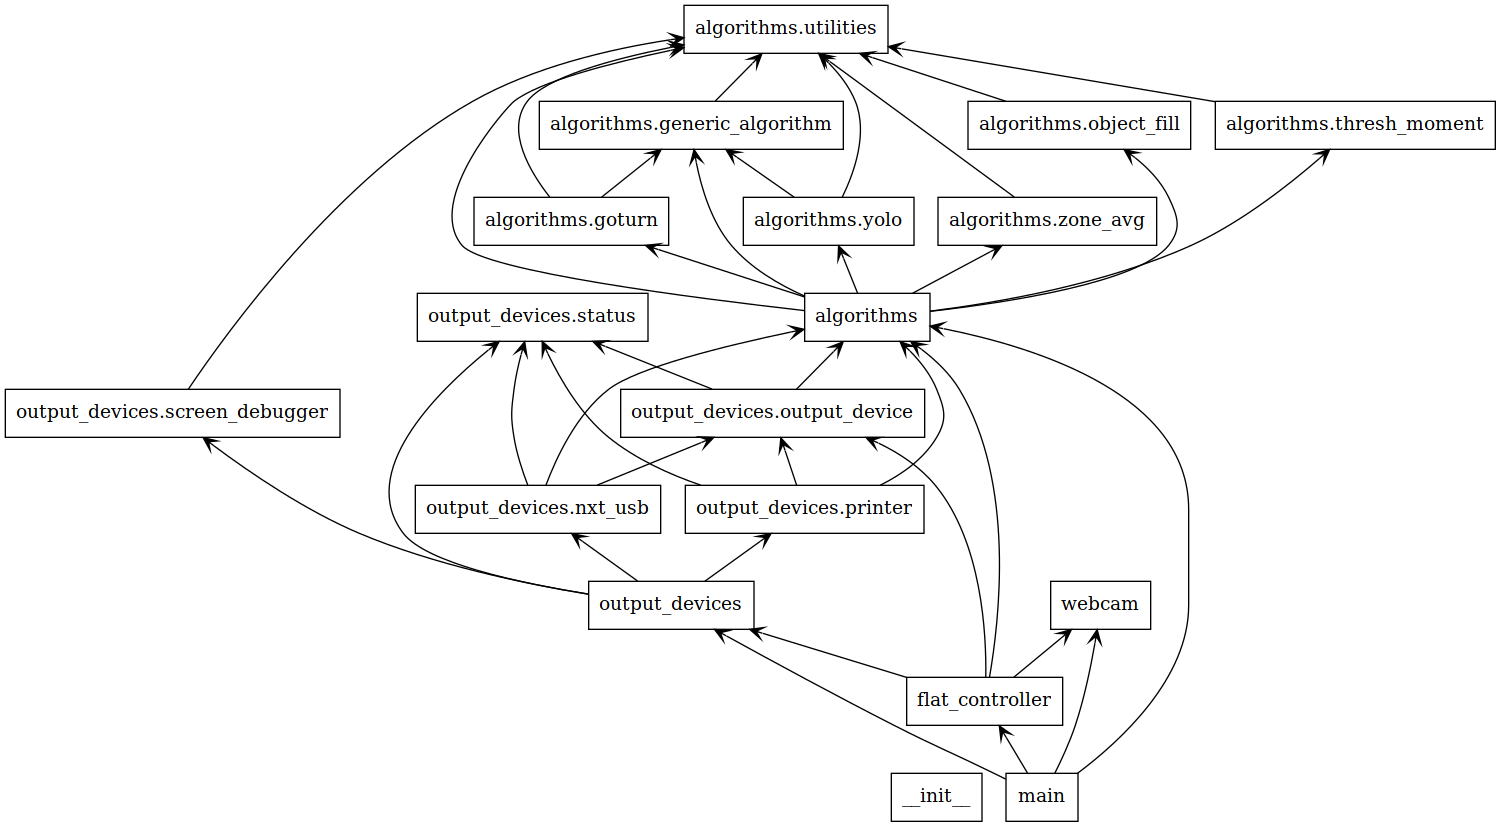
\includegraphics[width=\textwidth]{5.Solution/images/python_packages.png}
	\caption{The dependencies of the packages of the project{.} Image generated with pyreverse\cite{pyreverse}}
	\label{fig:pythonClasses}
\end{figure}


The project also contains functions for calibration, as seen on \autoref{fig:pythonClasses}, which will be covered in \autoref{sec:calibration}.

\subsection{Main.py}
The entry point for the python program is \texttt{main.py}.
The arguments for \texttt{main.py}  are shown in \autoref{lst:MainHelp}.
\begin{lstlisting}[label={lst:MainHelp},caption={The help message of the commandline interface}]
$ python3 main.py --help
usage: main.py [-h] [-a [name]] [-n [no_usb]]

Run the object detection part of the F.L.A.T system

optional arguments:
-h, --help            show this help message and exit
-a [name], --algorithm [name]
Choose which algorithm to run [ZONE_AVG, OBJ_FILL,
THRESH_MOMENT]. default='thresh_moment'
-n [no_usb], --no-usb [no_usb]
Whether to disable USB connection with the NXT.
default=False
\end{lstlisting}

The main objective of \texttt{main.py} is to determine which arguments to pass onto the \texttt{FlatController}.

\subsection{FlatController}\label{flatcontrollerimplementation}
The \texttt{FlatController} class manages the different modules of the Python part of the project and ties the Python part of the solution together
The signature of the \texttt{FlatController} is shown in \autoref{lst:FlatControllerInit}.

\begin{lstlisting}[language=Python,label={lst:FlatControllerInit},caption={Initialization method of the \texttt{FlatController} class}]
	def __init__(self,
		algorithm: Callable[[np.ndarray], Optional[Vector]],
		output_device: OutputDevice,
		input_device: VideoController,
		calibration_algorithm: Union[Callable[[OutputDevice], None], None] = None,
		debug=True
		) -> None:
\end{lstlisting}

The order of the parameters are not an indication of their relevance, but is rather based on the requirement of Python itself, as Python requires parameters with default parameters to be first in the signature of the methods.

The method takes a function, \texttt{algorithm} with an array as input and a vector as output.
The function is a specification of the specific algorithm to use for image recognition.
The array is the array of pixels in a given frame, while the vector is the center of the found object in the image.

The \texttt{output\_device} parameter, specifies how to output the location data.
This can be direct transmission of data to the NXT or it can use a video feed, which is used for debugging and getting the video output of the what the \texttt{F.L.A.T}'s camera.

The \texttt{input\_device} parameter specifies which device the video feed should be received from.
This is primarily a live video feed taken from the \texttt{F.L.A.T}'s camera, but can also be video file.
The video file option was primarily used for testing.

The \texttt{calibration\_algorithm} is relevant when connected to an NXT and calibration is needed.
The calibration algorithm will send a request to the NXT, asking it to begin calibrating, after which the \texttt{calibration\_algorithm} will wait for the arrival of the calibration data from the NXT.

The \texttt{calibration\_algorithm} handles this information depending on implementation, the default implementation is simply storing this data for later usage.

Finally, the \texttt{debug} parameter specifies whether the program is in debug mode.
When in debug mode, various relevant information is posted to the screen, along with a live video feed.
The information includes the current tick count, the current frames per second and the current location found.


\subsection{Object Localization}\label{solution:ObjectLocalization}
As mentioned in subsection~\ref{flatcontrollerimplementation} there are multiple implemented options for object localization algorithms.
%Hjælp den her sætning vvvv.
This subsection will describe the two primary algorithms, that were used throughout the development of the project.
\subsection{Object Fill algorithm}\label{solution:objfillalgo}

The core of the Object Fill algorithm is the actual "filling" part.
It can be seen in a stripped down version in listing~\ref{lst:objectfill}

\begin{lstlisting}[language=Python,label={lst:objectfill},caption={Stripped version of thresh moment from thresh\_moment.py}]
    def _fill_get_center(self, object_position: Vector, frame: np.ndarray, image_size: Vector) -> Optional[Vector]:
	    queue: Deque = deque()
	    queue.append(object_position)
	    self._blacklisted_pixels.add(object_position)
	    sum_outline = Vector(0, 0)
	    sum_redness = 0
	    sum_elements_in_outline = 0
	    
	    while queue:
		    element = queue.popleft()
		    pixel_redness = _redness(element.x, element.y, frame)
		    # is a bounding pixel
		    if pixel_redness < self.red_threshold:
			    sum_outline += element
			    sum_elements_in_outline += 1
		    
		    for neighbour in self._get_neighbours(element, image_size) - self._blacklisted_pixels:
			    sum_redness += pixel_redness
			    self._blacklisted_pixels.add(neighbour)
			    queue.append(neighbour)
	    
	    if sum_redness > DEFAULT_MIN_TOTAL_REDNESS:
		    return sum_outline / sum_elements_in_outline
	    else:
		    return None
\end{lstlisting}

A high level explanation of the algorithm can be found in Section~\ref{sec:objectfilldesign}.
\subsection{Thresh Moment Algorithm}\label{solution:thresh_moment}

A stripped down version of the Thresh Moment algorithm can be seen in listing~\ref{lst:threshmoment}, with inline comments.

\begin{lstlisting}[language=Python,label={lst:threshmoment},caption={Stripped version of thresh moment from thresh\_moment.py}]
	def locate_center(self, frame: np.ndarray) -> Optional[Vector]:
	    # Convert image to HSV
	    hsv_frame = cvtColor(frame, COLOR_BGR2HSV)
	    # Get mask from red threshold
	    mask = inRange(hsv_frame, (0, 150, 50), (10, 255, 255)) inRange(hsv_frame, (170, 150, 50), (180, 255, 255))
	    
	    # Find contours from mask
	    _, contours, _ = findContours(mask, RETR_TREE, CHAIN_APPROX_SIMPLE)
	    # Filter contours with areas that are considered too small to be the target
	    contours = [contour for contour in contours if contourArea(contour) > 20]
	    
	    if len(contours) != 0:
		    biggest_contour = max(contours, key=contourArea)
		    
		    # Find moment from the biggest contour
		    moment = moments(biggest_contour)
		    # Get center x and center y coordinate based on moment
		    cx = int(moment["m10"] / moment["m00"])
		    cy = int(moment["m01"] / moment["m00"])
		    return Vector(cx, cy)
	    return None
\end{lstlisting}

\section{Calibration}\label{sec:calibration}
As explained in \autoref{subsec:variablemotorpower} varying power was required depending on the current revolution of each motor, and the direction of movement.

To solve this problem, data was gathered for the minimum amount of power required to change the revolution.
This data was then processed in a neural network, finding a relation between power and revolution in each direction.
The neural network was then exported as C code and compiled on the NXT, and used as a base-value for motor power.

To collect the data for the power required to move 1 degree, a function was created on the NXT.
This function slowly increases power while checking for a change in the current revolution. 
A simplified version of the function can be seen in \autoref{lst:GetRequiredPower}.


\begin{lstlisting}[language=C,label={lst:GetRequiredPower},caption={Getting required power to move }]
int8_t get_power_to_move(T_AXIS_TYPE axis, T_DIRECTION direction) {
	int8_t power = MIN_POWER;
	T_REVOLUTION first_revolution = get_current_revolution();

	do {
		set_motor_speed(axis, power * (direction == POSITIVE ? 1 : -1));
		power++;

		// wait 30ms but make sure we don't move in that timeframe
		for(int i = 0; i < 30; i++)
		{
			systick_wait_ms(1);
			if (!should_stop_moving(first_revolution, power))
				break;
		}

	} while(should_stop_moving(first_revolution, power));

	set_motor_speed(axis, 0);

	return power;
}

\end{lstlisting}

The \texttt{should\_stop\_moving} function will determine whether the motor has moved, or if the power exceeds the maximum allowed power, meaning it is unable to move further.
The data is sent back to the host machine over the established USB connection.

%The function was run multiple times, and whenever the device was modified, the calibration function was run again.

An example data-set is shown on \autoref{fig:calibdata}.
This dataset is based on the y-axis in an upwards direction.

\figur{1}{images/calib_data.png}{Required power for revolution on motor}{fig:calibdata}

There is a clear tendency in the data, as the power requirements increases as the head of the device is raised.

Using this data, a neural network was trained to find the tendency of the data.
The training was done with the Python module, scikit-learn\cite{scikit-learn}, which exposes a regressor called \texttt{MPLRegressor}, which was utilized as shown in \autoref{lst:mlpregressor}.


As nxtOSEK was somewhat incompatible with parts of the \texttt{math.h} library from c, a custom activation function was required.

An approximation of the sigmoid function was implemented instead, both in Python and in C.

\begin{lstlisting}[language=python,label={lst:mlpregressor},caption={Training a MLPRegressor with scikit}]
model = MLPRegressor(
  hidden_layer_sizes=(30,),
  activation='approx_sigmoid',
  max_iter=100000,
  tol=0.0000001,
  verbose=True
)
model.fit(inp, expect)

\end{lstlisting}

\autoref{lst:mlpregressor} shows the initialization and fitting of the \texttt{MLPRegressor} 
A custom amount of hidden layers was required as the default argument value was 100 neurons in one layer, which was not necessary for the simple dataset.
30 neurons in one layer was decided upon after testing different layer sizes.

As mentioned, a custom approximation of the sigmoid function was used as the activation function, the maximum iterations was increased and the tolerance was increased, making the network run for longer, before terminating
This makes sure the network is good enough to be used in the system.

One of the networks created with 30 neurons is shown in \autoref{fig:calibdatann}, where the line is the result of the neural network.

The data is normalized to better work with the SGD function, using a preprocessor exposed by the scikit-learn module.

\figur{1}{images/calib_data_nn.png}{Sample fitting of the data}{fig:calibdatann}

\autoref{fig:calibdatann} shows the neural network for the upwards direction, however the same process was done simultaneously for the downwards direction.
Calibration was only done for the $Y$-axis.
A result from two calibrations and their associated function fittings are shown on \autoref{fig:calibdatannboth}.

\figur{1}{images/calib_data_nn_both.png}{Both neural networks of the $Y$ axis}{fig:calibdatannboth}

The weights and biases of the neural networks, were exported as C, and compiled to the NXT, along with the rest of the NXT code.
A simplistic version of an exported model in C is shown in \autoref{lst:exportedmodel}.


\begin{lstlisting}[language=C,label={lst:exportedmodel},firstnumber={1},caption={Autogenerated model for getting power to move up}]
#include <stdint.h>
#include <math.h>

typedef struct {
	double input_0;
} T_MODEL_INPUT;

typedef struct {
	double output_0;
} T_MODEL_EXECUTION_RESULT;

static double sigmoid(double value)
{
	double x = value >= 0 ? value : value * -1;
	double x2 = x * x;
	double e = 1.0f + x + x2 * 0.555f + x2 * x2 * 0.143f;
	return 1.0f / (1.0f + (value > 0 ? 1.0f / e : e));
}
static double WEIGHTS_LAYER_0[1][30] = {
	{ 0.6808517232629588, ...., 4.170499471133788 }
};
static double WEIGHTS_LAYER_1[30][1] = {
	{ 0.8428497309705472 },
	...
	{ -2.015815865114775 }
};
static double BIAS_LAYER_0[30] = {
	-0.8555370213729661, ...., 3.3193827456697775
};
static double BIAS_LAYER_1[1] = {
	0.09092457039425662
};
T_MODEL_EXECUTION_RESULT calculate_model_up(T_MODEL_INPUT input) {
	//calculate result
}

\end{lstlisting}

The function \texttt{calculate\_model\_up} normalizes the input data, and then calculates the output as explained in \autoref{sec:calculationsNN}.
Finally, the output value is denormalized in order to be used in the system.
This function is used in the movement module, to calculate the base power.
The specifics are explained in \autoref{sec:movement}.


\subsection{Python USB implementation}\label{sol:subsec:pythonusb}
%Denne er måske alt for detaljeret
In \autoref{sec:usbdes} the overall design of the USB communication was described.
The following subsection will describe how the USB communication is implemented in the Python part of the the solution.
The NXT specific USB implementation will be described in \autoref{sec:nxtusbimp}.

The USB device inherits from the OutputDevice base class.
The implementation uses the PyUSB library, as described in \autoref{sec:usbdes}\cite{PyUSB}.

\autoref{lst:PythonUSBInit} shows the initialization of the NxtUsb module, which handles the USB communication from Python to the NXT.
\begin{lstlisting}[label={lst:PythonUSBInit},caption={The initialization of PyUSB{.} Comments removed}]
def __enter__(self):
    self.device = usb.core.find(idVendor=ID_VENDOR_LEGO, idProduct=ID_PRODUCT_NXT)

    if self.device is None:
        raise DeviceNotFound('Device not found')

    self.device.set_configuration()

    self.out_endpoint, self.in_endpoint = self.device[0][(0, 0)]
    self.out_endpoint.write(b'\x01\xFF') 
    self.device.read(self.in_endpoint.bEndpointAddress, 8) 
    self.initialized = True
    return self
\end{lstlisting}

The code itself is relatively self-explanatory, and only the most interesting parts will be elaborated upon.
Line 9 sets the endpoint for the outgoing communication.
Incoming communication uses a secondary endpoint, which is found at the time of reading data.

At this point in the program, the NXT is waiting for a specific code, which is sent in line 10.

When the NXT receives the code, it returns \texttt{{.}ecrobot}.
Should that be the case, it sets its initialized field to \texttt{True} and returns.

With the device initialized, communication can now happen.
The communication itself is relatively simple, with the read method simply reading directly from the byte stream, as shown in \autoref{lst:PythonUSBread}.

\begin{lstlisting}[label={lst:PythonUSBread},caption={Reading from the USB port connected to the NXT}]
	def read(self) -> bytes:
		return self.device.read(self.in_endpoint.bEndpointAddress, 8)
\end{lstlisting}

When writing to the device, there are two options:
The first, \texttt{write\_location}, writes a location to the USB, while the second \texttt{write\_status}, writes a status.
Both are shown in \autoref{lst:PythonUSBwrite}.

\begin{lstlisting}[label={lst:PythonUSBwrite},caption={Writing from the USB port connected to the NXT}]

	
	def write_location(self, data: Tuple[Vector, bool]) -> None:
	
		loc, on_target = data
		self.out_endpoint.write(bytes([
			Status.ON_TARGET.value if on_target else Status.TARGET_FOUND.value,
			0,
			int(loc.x) & 0xFF,
			int(loc.y) & 0xFF
		]))
	
	def write_status(self, status: Status):
		value = status.value
		if type(value) is tuple:
			value = value[0]
		self.out_endpoint.write(bytes([
			int(value) & 0xFF,
			0
		]))

\end{lstlisting}
Both methods send byte wise data.

%\section{Cross platform communication}\label{solution:Communication}



\section{Mapping between computer vision and movement}
Two functions are needed to transfer the screen position to a velocity on the motors.
First we need to transfer the screen position to the USB transfer, and then that format to a motor velocity.

\subsection{Screen to motors}
Two functions are needed to transfer the screen position to a velocity on the motors.
First we need to transfer the screen position to the USB transfer, and then that format to a motor velocity.

We need to make a function on the python part that maps these numbers.

This function will take in 'pos` which is going to be a 2d vector.

We get a location on the screen that we want to transfer to a 8-bit value. 
The range on the screen is 0-480 on one axis and 0-640 on the other.
The range on the "out" is in theory 0-255, however as we, later, want to change this into an either positive or negative velocity (based on direction) we need to center it around 0 (that makes it easier atleast) so the value will be -127 - 127 (ignoring the -128 value that is in fact possible in the 8-bit range).


We will define two constants:
\begin{itemize}
\item in\_max = (480,640)
\item out\_max = 127
\end{itemize}

So we first need a function that maps the screen position to be zero centred: 
$$
in_\text{max}/2 - pos
$$

then we need to map this range to a new range, which we do by first translating the range from -240 - 320 to -1 - 1
this can be done with:
$$
in_\text{max}/2 - pos)/(in_\text{max}/2
$$


Then multiplying this value with the wanted out\_range.

$$
(in\_max/2 - pos)/(in\_max/2) \cdot out\_max
$$

This gets us a simple value between -127 and 127. However this grants us the same precision in the lower end of the scale as with the high end of the scale.
So when the target is far away, we get the same precision as when it is close, and one could argue that precision is more important closer to the center (when small but precise adjustments are needed).
For this exact reasoning, we will utilize the same principles as floating point precision, and make a Quadratic function. 

After tweaking around in Geogebra for some time, the following function was chosen.

$$
f(pos) = ((in_\text{max}/2 - pos)/(in_\text{max}/2))^2 \cdot out_\text{max}
$$

However a minor problem with this is that taking the position to the power of 2, removes the direction of the given axis (as -2 becomes 2)
so we times the whole thing with either -1 or 1 on each axis to keep the direction.

$$
f(pos) = ((in_\text{max}/2 - pos)/(in_\text{max}/2))^2 \cdot dir(pos) \cdot out_\text{max}
$$

\subsection{From USB to motors}
The NXT receives a vector in range (-127 -> 127, -127 -> 127).
This ought to get mapped to the speed of the motor which is a value of -100 and 100, on each axis.
Either full speed in the negatie direction or full speed in the positive direction.


The output of the USB is an 8 bit int, and the input of the motor is also an int.
The easiest way to do these calculations are simply mapping the ranges directly onto each other

However we never want full speed (as that is quite extreme) nor do we want 0 speed (as the motors oftentimes won't move before reaching a power of 10-20 due to sheer weight).
Therefore the actual range is something like -30 and -10 and 10 and 30

These values of $\pm10$ and $\pm30$ should obviously be tweakable, but in these examples, 10 and 30 will be used for the sake of examples. 
Input, in these constants, is the input of the function, which is the output of the USB module.

	lower\_bound = 10
	upper\_bound = 30
	input\_upperbound = 127
	range = upper\_bound - lower\_bound

normally mapping from input to output would be making the input into a range of -1 and 1, however this required floating point precision (otherwise we simply get -1, 0 or 1) so instead we do it in a bit of an other order.

$$
speed(pos) = (pos \cdot range)/input_\text{upperbound} + (dir(pos) \cdot lowerbound)
$$

An issue with direction rises again with direction, bacause of lowerbound.
This is fixed by using the direction, so we actually uses the bound correctly.
\section{USB implentation}
\label{sec:usbimp}
In Section~\ref{sec:usbdes}, a high level description of the USB communication between the computer and the NXT was described.
This section will describe the specifics of the implementation of the USB receiver on the NXT.

The USB receiver has 3 parts, which is also shown in Figure~\ref{fig:compusb}.

\begin{lstlisting}[language=CSharp,label={lst:usbhandshake},caption={ecrobot\_device\_initialize method from nxt.c}]
    void ecrobot_device_initialize(void) {
        init_motor(NXT_PORT_A, 'y', 20);
        init_motor(NXT_PORT_B, 'x', 20);
        ecrobot_init_usb();
    }
\end{lstlisting}
Snippet~\ref{lst:usbhandshake} shows the initializion of the NXT device.
\texttt{ecrobot\_device\_initialize} is invoked by nxtOSEK on program startup.
The essential function call for function call is the \texttt{ecrobot\_init\_usb()} call.
This function is a part of the nxtOSEK API and is required to use the NXT's USB port for communication.
As mentioned in Section~\ref{sec:usbdes}, this part posed a few challenges, as it was not clearly documented.

The next part of the USB receival is the actual continuous retrieval from the USB buffer.
\begin{lstlisting}[language=CSharp,label={lst:usbreceive},caption={get\_status\_code method from usb.c}]
bool get_status_code(STATUS_CODE *out_code, T_VECTOR *out_location) {
	int32_t len;
	uint8_t buffer[MAX_SIZE_OF_USB_DATA];

	/* critical section */
	GetResource(USB_Rx);
	/* read USB data */
	len = ecrobot_read_usb(buffer, 0, MAX_SIZE_OF_USB_DATA);
	ReleaseResource(USB_Rx);

	if (len == sizeof(STATUS_CODE))
	{
		memcpy(out_code, buffer, sizeof(STATUS_CODE));
		return true;
	}
	if (len == MAX_SIZE_OF_USB_DATA) {
		memcpy(out_code, buffer, sizeof(STATUS_CODE));
		memcpy(out_location, buffer + sizeof(STATUS_CODE), sizeof(T_VECTOR));
		return true;
	}
	return false;
}
\end{lstlisting}
The \texttt{get\_status\_code} function handles both the continous read of the USB and setting the status code of the system.

The \texttt{GetResource(USB\_Rx)} call, locks the USB resource for other processes.
It then reads the data from the USB buffer, with the \texttt{ecrobot\_read\_usb} call, into the data unsigned integer data and releases the USB resource.

After releasing the USB resource, the function checks the length of the data, which can be the length of a status code, which is defined as an unsigned 16 bit integer in the \texttt{usb.h} header file the length of \texttt{MAX\_SIZE\_OF\_USB\_DATA}.
In the case of a status code, this code is copied to the \texttt{out\_code} which is specified as an input parameter in the form of a pointer.
Alternatively, it can be of length \texttt{MAX\_SIZE\_OF\_USB\_DATA}, which is defined as a status code concatenated with a target vector, a data structure containing a set of x and y coordinates in the form of two 16 bit integers.
In this case, the status code is copied to the \texttt{out\_code} and the received target information is copied to the \texttt{out\_location}, which is also specified as an input parameter. 
If nothing is read from the USB, meaning that the length of the read data is $0$, it returns false to indicate that nothing was read.

The \texttt{get\_status\_code function} is called from the \texttt{receive\_data} function in the \texttt{nxt.c} file, which contains the tasks for the device.

\section{Movement module}
The movement module is responsible for making the turret move according to a target.
The module consists of multiple methods which are responsible for isolated areas of the overall function. 
In the following the movement module will be elaborated upon and some of the main methods will be explained. 

\subsection{The motors}
Before using the LEGO motors, the NXT needs to know which ports are used for each motor. 
This is done as follows:
\begin{lstlisting}[language=CSharp, label={lst:DeviceInit},caption={ecrobot\_device\_initialize method from movement.c}]
void ecrobot_device_initialize(void){
  init_motor(NXT_PORT_A, 'x', 20);
  init_motor(NXT_PORT_B, 'y', 20);
}
\end{lstlisting}
As it ca be seen on Snippet~\ref{lst:InitMotor} the port on the NXT is specified with an orientation and an initial speed.
The \textit{init\_motor} method is declared as follows where the different parameters of the motor function is set up with initial values.

\begin{lstlisting}[language=CSharp,label={lst:InitMotor},caption={init\_motor method from movement.c}]
bool init_motor(uint8_t motor_id, char orientation, uint16_t speed){
  if(orientation == 'x'){
    x_motor = motor_id;
    x_motor_speed = speed;
    ecrobot_set_motor_speed(x_motor, 0);
    nxt_motor_set_count(x_motor, 0);
    current_location.x = ecrobot_get_motor_rev(motor_id);
    return true;
  }
  else if(orientation == 'y'){
    y_motor = motor_id;
    y_motor_speed = speed;
    ecrobot_set_motor_speed(y_motor, 0);
    nxt_motor_set_count(y_motor, 0);
    current_location.y = ecrobot_get_motor_rev(motor_id);
    return true;
  }
  return false;
}
\end{lstlisting}
As it can be seen on Snippet~\ref{lst:DeviceInit} line 2 and 3 the parameter for the motor\_id is the port id on the NXT device. 
The character for orientation of the motor is used to distinguish between the two motors as they are connected to the NXT.
The speed is set to an initialization value of $20$ which can be any given value between $0$ and $100$.

\subsection{The motion}
Before any meaningful motion can be made it is essential to know where the turret is currently aiming and where the target is located. 
Without this information any motion will result in a meaningless motion and should therefore be avoided. 

When the machine intelligence system has found and located the target it will send the information to the NXT and the NXT will then start to aim at the target. 
The target location is stored in an struct containing all relevant information about the target. 
The move\_motors method is responsible for the actual activation of the individual motors.
The method can be seen on Snippet~\ref{lst:MoveMotors} and it will activate the motors according to the targets location and where it is currently aiming. 
\begin{lstlisting}[language=CSharp,caption={move\_motors method from movement.c},label={lst:MoveMotors}]
void move_motors(){
  current_location.x = ecrobot_get_motor_rev(x_motor);
  current_location.y = ecrobot_get_motor_rev(y_motor);

  if(current_location.x > target_location.x){
    ecrobot_set_motor_speed(x_motor, -x_motor_speed);
  }
  else if(current_location.x < target_location.x){
    ecrobot_set_motor_speed(x_motor, x_motor_speed);
  }
  if(current_location.y > target_location.y){
    ecrobot_set_motor_speed(y_motor, -y_motor_speed);
  }
  else if(current_location.y < target_location.y){
    ecrobot_set_motor_speed(y_motor, y_motor_speed);
  }
}
\end{lstlisting}
Once the motors has engaged and the turret is aiming at the target, the motion should be stopped. 
If power is simply removed from the motors the motor will loos their stiffness and the entire turret will power down. 
To avoid this the motors has a function to simply set the speed of the motors to $0$ resulting in the motors locking up since they will actively try to counter act any motion. 
As shown on Snippet~\ref{lst:StopMotors} this method is very simple but effective. 
\begin{lstlisting}[language=CSharp,label={lst:StopMotors},caption={stop\_motors method from movement.c}]
void stop_motors(){
  nxt_motor_set_speed(x_motor, 0, 1);
  nxt_motor_set_speed(y_motor, 0, 1);
}
\end{lstlisting}

\subsection{Summery}
Based on the methods described above the Lego turret is able to move based on the input given by the machine intelligence. 
Hence the purpose of the movement module is to facilitate the movement of the turret which has thereby been accomplished. 



































\section{Scheduling}\label{solution:scheduling}
The scheduling of the system was first implemented as cyclic executive.
On \autoref{lst:MainTask} the implementation of the main task of the system is shown.
The main task is responsible for the scheduling of the system.

This task consists of two loops that correspond to the two states that the system can operate in: calibrating and normal execution.
As can be seen on \autoref{lst:MainTask} lines 3 to 12 the calibration state has to be completed before the system can start the normal execution.
On lines 13 to 25 the actual scheduling of all the needed methods can be seen, these method will be called once per major cycle hence being true to the deadline.

\begin{lstlisting}[language=CSharp,label={lst:MainTask},caption={MainTaks method from logic.c}]
TASK(MainTask)
{
    for (;;) {
        calibrating = true;
        show_init_screen();
        while(!get_status_code(&current_status, 0));

        if (current_status == READY_FOR_CALIBRATION)
        {
            calibrate(false);
        }
        calibrating = false;
        for(;;)
        {
            WaitEvent(newMajorCycleEvent);
            keep_USB_alive();
            receive_data();
            if (current_status == DISCONNECTED_REQ) {
                stop();
                break;
            }
            move_motors();
            handle_laser();
            update_display();
            ClearEvent(newMajorCycleEvent);
        }
    }
    TerminateTask();
}
\end{lstlisting}

In order to time the major cycle, the \textit{user\_1ms\_isr\_type2} method, that can be seen on \autoref{lst:user1msisrtype2}, is used to raise the event of the major cycle.
The method is activated by a system interrupt, ensuring that the method will be called once every millisecond.
\begin{lstlisting}[language=CSharp,label={lst:user1msisrtype2},caption={user\_1ms\_isr\_type2 method from nxt.c}]
void user_1ms_isr_type2(void)
{
    (void)SignalCounter(SysTimerCnt);
    SetEvent(MainTask, newMajorCycleEvent);
    if(calibrating)
        keep_USB_alive();
}
\end{lstlisting}

As part of the implementation of the cyclic executive scheduling method, an event is waiting to be raised after each cycle iteration.
On \autoref{lst:newMajorCycleEvent} the event is specified on the operation system level, such that it can be raised by the interrupt.
\begin{lstlisting}[language=CSharp,label={lst:newMajorCycleEvent},caption={newMajorCycleEvent event from nxt.oil}]
EVENT newMajorCycleEvent{
    MASK = AUTO;
};
\end{lstlisting}

The system only has one task, which is declared with the properties shown on \autoref{lst:MainTask}.
The properties specifies to the operating system how the task shall run and that the event from before is related to the task.
\begin{lstlisting}[language=CSharp,label={lst:MainTaskoil},caption={MainTaks task from nxt.oil}]
    TASK MainTask {
      AUTOSTART = TRUE
        {
          APPMODE = appmode1;
        };
      PRIORITY = 1;
      ACTIVATION = 1;
      SCHEDULE = FULL;
      STACKSIZE = 512;
      RESOURCE = USB_Rx;
      EVENT = newMajorCycleEvent;
};
\end{lstlisting}

The reasoning behind having a major cycle with no minor cycles is the execution time of the individual methods, which can be seen on \autoref{table:executionTimes1}.

\begin{table}[H]
\begin{tabular}{lll}
\textbf{Task name}  & \textbf{Execution time} & \textbf{Deadline} \\
Keep\_USB\_Alive    & 16     	& 1000                    \\
Receive\_Data       & 13       & 1000                    \\
Move\_Motors        & 12116    & 15000                   \\
Handle\_Lasers      & 6        & 1000                    \\
Update\_Display     & 267      & 15000                   \\
Background\_Task	 & 0	    & 15000					   \\
\end{tabular}
\end{table}\label{table:executionTimes1}

Since the execution time of all the tasks totals to a mere 535 microseconds, it was deemed non-essential to include minor cycles, as the tasks all depend on receiving new data from the USB, and this will not occur more than once every millisecond due to hardware limitations.
Likewise, there is a software limitation when using nxtOSEK, since the interrupt service routine is only run once every millisecond.
With these considerations, the cyclic execution method with equal minor and major cycles were deemed the best solution, since the implementation of a fixed priority task would add more overhead when changing between tasks and preempting them, rather than just allowing the previous tasks to finish executing.

\subsection{Fixed Priority Scheduling}
However, as the project progressed, parts of the machine intelligence execution were moved to the NXT for execution.
This resulted in tasks that took longer than 1 millisecond to execute, rendering the use of cyclic executive unviable, as described in \autoref{Design:Scheduling}.
Instead, the fixed-priority scheduling model was utilized.

After having added machine learning to the \texttt{Move\_Motors} task the execution times are as follows:

\begin{table}[H]
\begin{tabular}{lll}
\textbf{Task name}  & \textbf{Execution time} 	& \textbf{Priority}\\
Keep\_USB\_Alive    & 16                        & 4   \\
Receive\_Data       & 13                        & 3   \\
Move\_Motors        & 12116                     & 2   \\
Handle\_Lasers      & 6                         & 4   \\
Update\_Display     & 267                       & 1   \\
Background\_Task    & 0                         & 0   
\end{tabular}
\end{table}\label{table:executionTimes1}

As the cyclic executive approach allowed running the calibration before entering the first major cycle, this was easily implemented.
However, this does not work with the fixed-priority scheduling model, as the tasks are repeatedly run according to their tasks.
To fix this, the \texttt{Background\_Task} was introduced, which has a high enough priority to preempt the other tasks on the system to allow calibration to run, while still keeping the USB connection alive.

\begin{lstlisting}[language=CSharp,label={lst:backgroundTask},caption={Background task}]
TASK(background_task) {
  if(!calibrated) {
    show_init_screen();
    while(!get_status_code(&current_status, 0));

    if (current_status == READY_FOR_CALIBRATION) {
      calibrate(false);
    }
    calibrated = true;
  }
  if (current_status == DISCONNECTED_REQ) {
    stop();
  }
  TerminateTask();
}
\end{lstlisting}

As seen in \autoref{lst:backgroundTask}, the task checks if the boolean value, calibrated, is true.
Calibrated indicates if calibration is completed.
If this is not the case, the background task ensures that the status of the motors and USB are set as disconnected using the \texttt{stop} function.

In the cyclic executive model, it was ensured that the \texttt{keep\_USB\_alive} task was executed once every millisecond by running it at the beginning of each cycle, as the cycles had a length of 1 millisecond.
With the FPS model, this is instead done by assigning the \texttt{keep\_USB\_alive} task with the highest possible priority.
This ensures that it will run ahead of all other tasks, using preemption if needed.
To further ensure that it is run exactly once every 1 millisecond, an alarm is specified in the OIL file, as seen in \autoref{lst:OILAlarm}.

\begin{lstlisting}[language=CSharp,label={lst:OILAlarm},caption={Alarm in the OIL}]
/* Definition of keep_USB_alive execution timing */
ALARM cyclic_keep_USB_alive
{
  COUNTER = SysTimerCnt;
  ACTION = ACTIVATETASK
  {
    TASK = keep_USB_alive;
  };
  AUTOSTART = TRUE
  {
    ALARMTIME = 1;
    CYCLETIME = 1; /* keep_USB_alive is executed every msec */
    APPMODE = appmode1;
  };
};
\end{lstlisting}

The \texttt{counter} attribute specifies that the system clock is used to time when the alarm should be run, and which action it should take upon activation.
In the autostart block, it is defined that the cycle time is 1, meaning that the task will run once every 1 update of the SysTimerCnt, which happens once every 1 millisecond, thus ensuring that the task will run every millisecond.

The remaining tasks are set to automatically start, and will be allowed to run based on their priority with no pre-defined release time.

\section{Build process}\label{sec:buildprocess}
The build process for the project is quite complex as it targets the NXT.
This complicates the build process for a number of reasons:
nxtOSEK is the operating system for RTS on the NXT, and even though it is quite old, the latest release, as of the writing of this report, was released in January of 2013\cite{osekrelease}.
Additionally the nxtOSEK build process has a number of additional requirements.

During the groups testing of the nxtOSEK build, it was found that it was largely incompatible with modern operating systems, both Windows, OS X and a number of modern Linux distributions.
According to the latest documentation on the nxtOSEK webpage, the latest supported version of Linux is Ubuntu 11.10 which was released in 2011.
This complicated things a bit, as none of the group members were interested in installing such an old operating system on their personal computer, and instead Docker was used to avoid this.

\subsection{Docker}\label{subsec:docker}
Docker is a way to deploy a consistent environment for applications to run in, also known as containerization\cite{dockerdocstart}.
A Docker deployment consists of three different concepts, the Docker file, the container and an image.
\begin{description}
    \item [Dockerfile] which is a definition of a Docker image.
    \item [Images] are executables that includes all the required information to instantiate containers.
    \item[Containers] are the runtime instances of an image, the running process of an image.
\end{description}

A Dockerfile consists of lines, that describe how to build the image.
Each line applies a layer to the Docker image, and each of these layers are cached.
Thus if line 5 in the Dockerfile is changed, everything below line 5 is rebuilt.

The Dockerfile for this project is shown below, in \autoref{subsec:dockerimplementation}.

The Docker image is an executable, that instantiate a Docker container.

A Docker container is in broad strokes the same as a virtual machine, although a Docker container only uses the required resources, while a virtual machine is allowed access to more resources than is typically needed.
Docker runs natively on Linux, and takes no more memory than other executables.

The concept of containerization as a way to ensure consistency in deployment of software, was perfect for the purposes of the group.
Docker is supported on all 3 major platform, and while both Docker for Windows and MacOS run in a virtual machine, this is a non-issue.

A potential issue was nxtOSEK not being officially supported past Ubuntu 11.10, and Docker officially supporting Ubuntu 18.04, 16.04 and 14.04 \cite{dockerubuntu}.

This proved to be a non-issue, as modifying dependencies, and some tweaking, nxtOSEK ended up working fine on Ubuntu 14.04.

\subsection{Docker implementation}\label{subsec:dockerimplementation}
The actual Docker build process is somewhat obscure.

The first step is relatively straightforward with \textit{FROM ubuntu:14.04} specifying the base Ubuntu image to use.
The next bit installs the packages required by nxtOSEK.
\begin{lstlisting}[language=docker,label={lst:dockerimplementation1},caption={Version definition and installation of packages required by nxtOSEK}]
FROM ubuntu:14.04

# Install required packages listed by nxtOSEK
RUN apt-get update
RUN apt-get -y install tk-dev ncurses-dev libmpfr-dev wget gzip tar software-properties-common xvfb
\end{lstlisting}

The next part is the most obscure part, as wine is installed to be able to run Windows programs.
This is done as the tool to build OIL files, only exists for Windows.
NeXT Tools is an utility program that includes various utilities for use with nxtOSEK, including an enhanced OIL file compile\cite{nxttool}.
It also includes an additional nxtOSEK requirement, texinfo, which is the official GNU documentation format\cite{texinfo}.

The version of texinfo on the apt repository was not compatible, hence why a specific version was downloaded.

\begin{lstlisting}[language=docker,label={lst:dockerimplementation2},caption={Installation of Wine and texinfo},firstnumber=6]
# Install wine
RUN dpkg --add-architecture i386
RUN wget -nc https://dl.winehq.org/wine-builds/Release.key
RUN apt-key add Release.key
RUN apt-add-repository https://dl.winehq.org/wine-builds/ubuntu/
RUN apt-get -y install apt-transport-https
RUN apt-get update
RUN apt-get -y install --install-recommends winehq-staging

# Download a specific version of texinfo, the one in 14.04
# sources is not compatible with the expected version
RUN wget http://ftp.gnu.org/gnu/texinfo/texinfo-4.13.tar.gz
RUN gzip -dc < texinfo-4.13.tar.gz tar -xf -
RUN cd texinfo-4.13 \&\& ./configure \&\& make \&\& make install
\end{lstlisting}
Next, the ARM tool chain is installed.
The tool chain is used by nxtOSEK to build for the ARM7 CPU in the NXT.
\begin{lstlisting}[language=docker,label={lst:dockerimplementation3},caption={Building the ARM toolchain},firstnumber=20]
# Build arm toolchain from nxtOSEK
COPY build_arm_toolchain.sh home/
RUN chmod 755 home/build_arm_toolchain.sh
RUN home/build_arm_toolchain.sh

# Add build.sh
WORKDIR /home/nxtosek
COPY build.sh ./
RUN chmod 755 ./build.sh
\end{lstlisting}

Finally, the nxtOSEK files are moved to the home folder, before the entry point for the container is set to the location in the home folder.
This means that whenever the Docker image is run, any arguments are passed along to the build file in the home directory.

\begin{lstlisting}[language=docker,label={lst:dockerimplementation4},caption={Moving the nxtOSEK files and setting the entry point},firstnumber=29]
# Move nxtOSEK files to home folder
RUN useradd nxtosek
RUN usermod --password $(echo nxtosek openssl passwd -1 -stdin) nxtosek
RUN chown -R nxtosek ./
USER nxtosek
ENV HOME /home/nxtosek
ADD nxtOSEK.tar.xz ./
ADD ecrobot.mak nxtOSEK/ecrobot

# Set build.sh as entrypoint to execute when executing docker container
ENTRYPOINT ["/home/nxtosek/build.sh"]
CMD []
\end{lstlisting}

The Docker container allows the group to easily build the NXT implementation from any machine, as long as Docker is supported by the OS.
The Docker image is hosted publicly on the Docker Hub at \url{https://hub.docker.com/r/teknight/nxtosek/}.

In addition to local builds, the Docker image is also used on the TeamCity server, as part of the continuous integration for the project, meaning that the Docker image is used every time something is pushed to a branch.
%Maybe describe Continuous integration?

\subsection{Continous Integration}
To ensure that builds are not failing, the group set up a TeamCity server\cite{TeamCityHomepage} and combined it with GitHub Webhooks.
A GitHub webhook is sent from GitHub to the TeamCity server whenever new code has been pushed.
GitHub then provides a API endpoint for marking commits and branches as passing or failing builds, via their Status API \cite{GithubStatusAPI}.

\figur{1.0}{images/flowchart-build.png}{Our build-flow}{fig:flowchart-build}

To avoid a unmaintainable test-script, the build-process is split into sub-processes, such as the test-report script in \autoref{lst:pythonreportcheck}, that checks each line in \LaTeX{}-code for multiple sentences on a single line.
A test for this was introduced to reduce merge conflicts, as well as increasing readability.

\begin{lstlisting}[language=python,label={lst:pythonreportcheck},caption={Checking .tex files}]
#!/usr/bin/python

import os
import sys
import glob

white_list = ["eg", "i.e", "etc", "e.g"]

def get_tex_lines():
    for file in glob.iglob(os.path.dirname(os.path.realpath(__file__)) + '/report/*/**/*.tex', recursive=True):
        with open(file) as f:
            for line in f.readlines():
                yield line

def check_line(line, initial = True):
    parts = line.strip().split("(*@{.}@*) ")
    if line.startswith("%"):
        return True
    if len(parts) == 1:
        return True if (initial or "." not in parts[0]) else any(parts[0][:-1].endswith(x) for x in white_list)

    newLine = "(*@{.}@*) ".join(parts[:-1])
    for x in white_list:
        if newLine.endswith(x):
            return check_line(newLine[:-len(x)], False)
    return False

result = True
for line in get_tex_lines():
    if not check_line(line):
        print("Illegal line:", line)
        result = False

exit(0) if result else exit(1)
\end{lstlisting}

One of the advantages of using a continuous integration tool is that the merging is self-testing.
This means that when maintaining smaller code changes, that are merged into a mainline branch often, instead of monolithic merges, that have a higher likelihood of conflicting code, and long running forks.

Overall, the continuous integration has helped to ensure that unit tests were always passing and that the mainline branch is working.
This is done by running through the flowchart in \autoref{fig:flowchart-build} every time some code needs to be build.
This includes building the NxtOSEK program, ensuring no compile time errors and compile the \LaTeX{} code as well.

